% This is "sig-alternate.tex" V2.1 April 2013
% This file should be compiled with V2.5 of "sig-alternate.cls" May 2012
%
% This example file demonstrates the use of the 'sig-alternate.cls'
% V2.5 LaTeX2e document class file. It is for those submitting
% articles to ACM Conference Proceedings WHO DO NOT WISH TO
% STRICTLY ADHERE TO THE SIGS (PUBS-BOARD-ENDORSED) STYLE.
% The 'sig-alternate.cls' file will produce a similar-looking,
% albeit, 'tighter' paper resulting in, invariably, fewer pages.
%
% ----------------------------------------------------------------------------------------------------------------
% This .tex file (and associated .cls V2.5) produces:
%       1) The Permission Statement
%       2) The Conference (location) Info information
%       3) The Copyright Line with ACM data
%       4) NO page numbers
%
% as against the acm_proc_article-sp.cls file which
% DOES NOT produce 1) thru' 3) above.
%
% Using 'sig-alternate.cls' you have control, however, from within
% the source .tex file, over both the CopyrightYear
% (defaulted to 200X) and the ACM Copyright Data
% (defaulted to X-XXXXX-XX-X/XX/XX).
% e.g.
% \CopyrightYear{2007} will cause 2007 to appear in the copyright line.
% \crdata{0-12345-67-8/90/12} will cause 0-12345-67-8/90/12 to appear in the copyright line.
%
% ---------------------------------------------------------------------------------------------------------------
% This .tex source is an example which *does* use
% the .bib file (from which the .bbl file % is produced).
% REMEMBER HOWEVER: After having produced the .bbl file,
% and prior to final submission, you *NEED* to 'insert'
% your .bbl file into your source .tex file so as to provide
% ONE 'self-contained' source file.
%
% ================= IF YOU HAVE QUESTIONS =======================
% Questions regarding the SIGS styles, SIGS policies and
% procedures, Conferences etc. should be sent to
% Adrienne Griscti (griscti@acm.org)
%
% Technical questions _only_ to
% Gerald Murray (murray@hq.acm.org)
% ===============================================================
%
% For tracking purposes - this is V2.0 - May 2012

\documentclass[]{acmlarge}
\usepackage[utf8]{inputenc}
\usepackage{pdflscape}
\usepackage{xcolor}
\usepackage{framed}
\usepackage{caption}

\makeatletter
\def\runningfoot{\def\@runningfoot{}}
\def\firstfoot{\def\@firstfoot{}}
\makeatother

\markboth{P. Silva, R. Monge and E B. Fernandez}{A Reference Architecture for web browsers: Part II, A pattern for Web Browser Content Renderer}
\colorlet{shadecolor}{gray!10}
% Metadata Information

\acmArticle{-}
 
 

% % Copyright
% \setcopyright{rightsretained}



% Copyright
%\setcopyright{acmcopyright}
\setcopyright{acmlicensed}
%\setcopyright{rightsretained}
%\setcopyright{usgov}
%\setcopyright{usgovmixed}
%\setcopyright{cagov}
%\setcopyright{cagovmixed}


% DOI
%\doi{10.475/123_4}

% ISBN
%\isbn{123-4567-24-567/08/06}

%Conference
%\conferenceinfo{EuroPLoP 2016}{July 6-10, Bavaria, Germany.}

%\acmPrice{\$15.00}

%
% --- Author Metadata here ---

%\CopyrightYear{2007} % Allows default copyright year (20XX) to be over-ridden - IF NEED BE.
%\crdata{0-12345-67-8/90/01}  % Allows default copyright data (0-89791-88-6/97/05) to be over-ridden - IF NEED BE.
% --- End of Author Metadata ---

\title{A Reference Architecture for web browsers: Part II, A pattern for Web Browser Content Renderer}
%\subtitle{[Extended Abstract]
%\titlenote{A full version of this paper is available as
%\textit{Author's Guide to Preparing ACM SIG Proceedings Using
%\LaTeX$2_\epsilon$\ and BibTeX} at


%\numberofauthors{3} %  in this sample file, there are a *total*
% of EIGHT authors. SIX appear on the 'first-page' (for formatting
% reasons) and the remaining two appear in the \additionalauthors section.
%

\author{
%\alignauthor
Paulina Silva and Raúl Monge
  \affil{Universidad Técnica Federico Santa María}
  %\affil{Valparaíso, Chile}\\
  %\email{pasilva@alumnos.inf.utfsm.cl}
% 2nd. author
%\alignauthor
  %\affil{Valparaíso, Chile}\\
  %\email{rmonge@inf.utfsm.cl}
% 3rd. author
%\alignauthor 
Eduardo B. Fernandez
  \affil{Florida Atlantic University}
  %\affil{Boca Raton, Fl, USA}\\
  %\email{fernande@fau.edu}
}

\begin{abstract}
Currently, most software developments are focused in creating systems connected to the Internet, which allows to add functionality within a system and facilities to their \textit{stakeholders}. This leads to depend on a \textit{web client}, such as a \textit{web browser}, which allows access to Internet services, data or operations that a system delivers. Within the browser's main components, a \textit{rendering engine} is in charge of obtaining a convenient data structure as an output for a \textit{browser process}.
%which at the same time will send this output to the \textit{operating system} and then showing it to the user through a \textit{display}. 
%If the output is a web page, it will be shown to the user as a graphical representation; if not, the information obtained by the resource will be saved in a format to the user's convenience. 
%The Internet influences the attack surface of the system, and unfortunately many stakeholders and developers are not aware of the risks to which they are exposed. The lack of security education among software developers and mainly the scarce and scattered documentation for browsers (and standardization) could become a big problem in large architectural developments that depend on browsers to perform their services. 
%A Reference Architecture (RA) of the \textit{web browser}, using Architectural Patterns, could be a starting point for understanding its security mechanisms and architecture, which interact with a bigger web systems. This architecture would unify ideas and terminology, giving a holistic view of implementation independent details for both the browser and the system it communicates with. To our best knowledge, we have not found documentation that could unify the mentioned ideas. 
We developed a Web Browser Communication pattern that describes the infrastructure to allow the communication between a web client (or a web browser) and a server in the Internet. In this paper, we describe the component in charge of the rendering for a obtained web resource within the web browser, named here as \textbf{Web Browser Content Renderer}. In this work we have described this component as a pattern, to describe how a browser's \textit{rendering engine} works and interacts with other subsystems. Patterns combine experience and good practices to obtain models that can be used for new designs, to compare and select systems/applications or to teach others. The audience to which our paper is focused are browser developers, web application developers, researchers and teachers, being the first two the most important. %Since the appearance of Google Chrome and the loosely-coupled architecture of Internet Explorer came out, the structure of a browser has evolved with the objective of making it faster, simpler and more secure for users. 
\end{abstract}


%
% The code below should be generated by the tool at
% http://dl.acm.org/ccs.cfm
% Please copy and paste the code instead of the example below. 
%


\keywords{Browser, Web Client, Browser Renderer, Reference Architecture, Pattern}
\acmformat{Paulina Silva, Raul Monge, and Eduardo B. Fernandez. 2016. A Reference Architecture for web browsers: Part II, A pattern for Web Browser Content Renderer}


\begin{document}
\acmYear{2016} 
\setcopyright{acmlicensed}
%\conferenceinfo{EuroPLoP '16,}{July 06 - 10, 2016, Kaufbeuren, Germany}
%\issn{978-1-4503-4074-8/16/07}\acmPrice{\$15.00}
\doi{http://dx.doi.org/10.1145/3011784.3011813}

\begin{CCSXML}
<ccs2012>
<concept>
<concept_id>10011007.10010940.10010971.10010972</concept_id>
<concept_desc>Software and its engineering~Software architectures</concept_desc>
<concept_significance>500</concept_significance>
</concept>
<concept>
<concept_id>10011007.10010940.10010971.10011120.10010538</concept_id>
<concept_desc>Software and its engineering~Client-server architectures</concept_desc>
<concept_significance>500</concept_significance>
</concept>
<concept>
<concept_id>10011007.10011006.10011008.10011024.10011036</concept_id>
<concept_desc>Software and its engineering~Patterns</concept_desc>
<concept_significance>500</concept_significance>
</concept>
</ccs2012>
\end{CCSXML}

\ccsdesc[500]{Software and its engineering~Software architectures}
\ccsdesc[500]{Software and its engineering~Client-server architectures}
\ccsdesc[500]{Software and its engineering~Patterns}
 

\begin{bottomstuff}
EuroPLoP '16, July 06 - 10, 2016, Kaufbeuren, Germany
\end{bottomstuff}

\maketitle

\section{Introduction}
Patterns are encapsulated solutions to recurrent problems and define a way to express requirements and solutions concisely, as well as providing a communication vocabulary for designers \cite{gamma1994design,buschman1996system}. The description of architectures using patterns makes them easier to understand, provides guidelines for design and analysis, and can define a way of making their structure more secure.

A Reference Architecture (RA) is created by capturing the essentials of existing architectures and by taking into account future needs and opportunities, ranging from specific technologies, patterns and business models. The aim of a RA is to provide a guide for developers, %who are not security experts, 
to develop architectures for concrete versions of some system or to extend such system. We are trying to describe the browser architecture as a RA composed  of architectural patterns. The pattern diagram \cite{buschman1996system} in Figure \ref{fig:relations} shows the relationships between our created patterns and we can see how different models relate to each other, where rounded rectangles represent patterns and the arcs indicate dependencies between patterns; for example, Interception of Traffic describes traffic threats.

    \begin{figure*}[h!t]
      \vspace*{-0.4cm}
      \centering
      \hspace{0.5cm}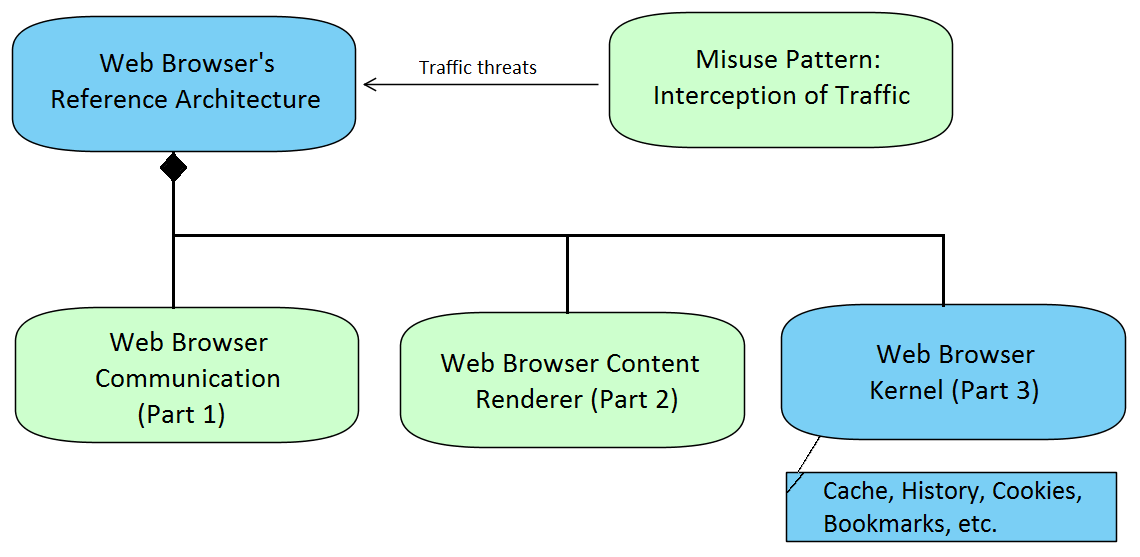
\includegraphics[scale=0.45]{figures/relations-finish.png}
      \caption{Pattern Diagram of our current work on the Reference Architecture for the Web Browser. Finished patterns in green and still developing in blue.}
      \label{fig:relations}
    \end{figure*}


Since we started to build our Reference Architecture (Figure \ref{fig:relations}), we are extending it by creating new architectural patterns for our RA and misuse patterns to describe threats and security patterns to build a Security Reference Architecture (SRA). We are currently building a SRA, which is a Reference Architecture where security services have been added in appropriate places to provide some degree of security for a specific system. The basic approach we will use to build a SRA is the application of a systematic methodology from \cite{fernandez2006methodology,Fernandez2011,Fernandez2016}, which can be used as a guideline to build secure web browser systems and/or evaluate their security levels. By checking if a threat, expressed as a misuse pattern, can be stopped or mitigated in the security reference architecture, we can evaluate its level of security.

    % \begin{figure*}[h!the]
    %   \vspace*{-1.5cm}
    %   \centering
    %   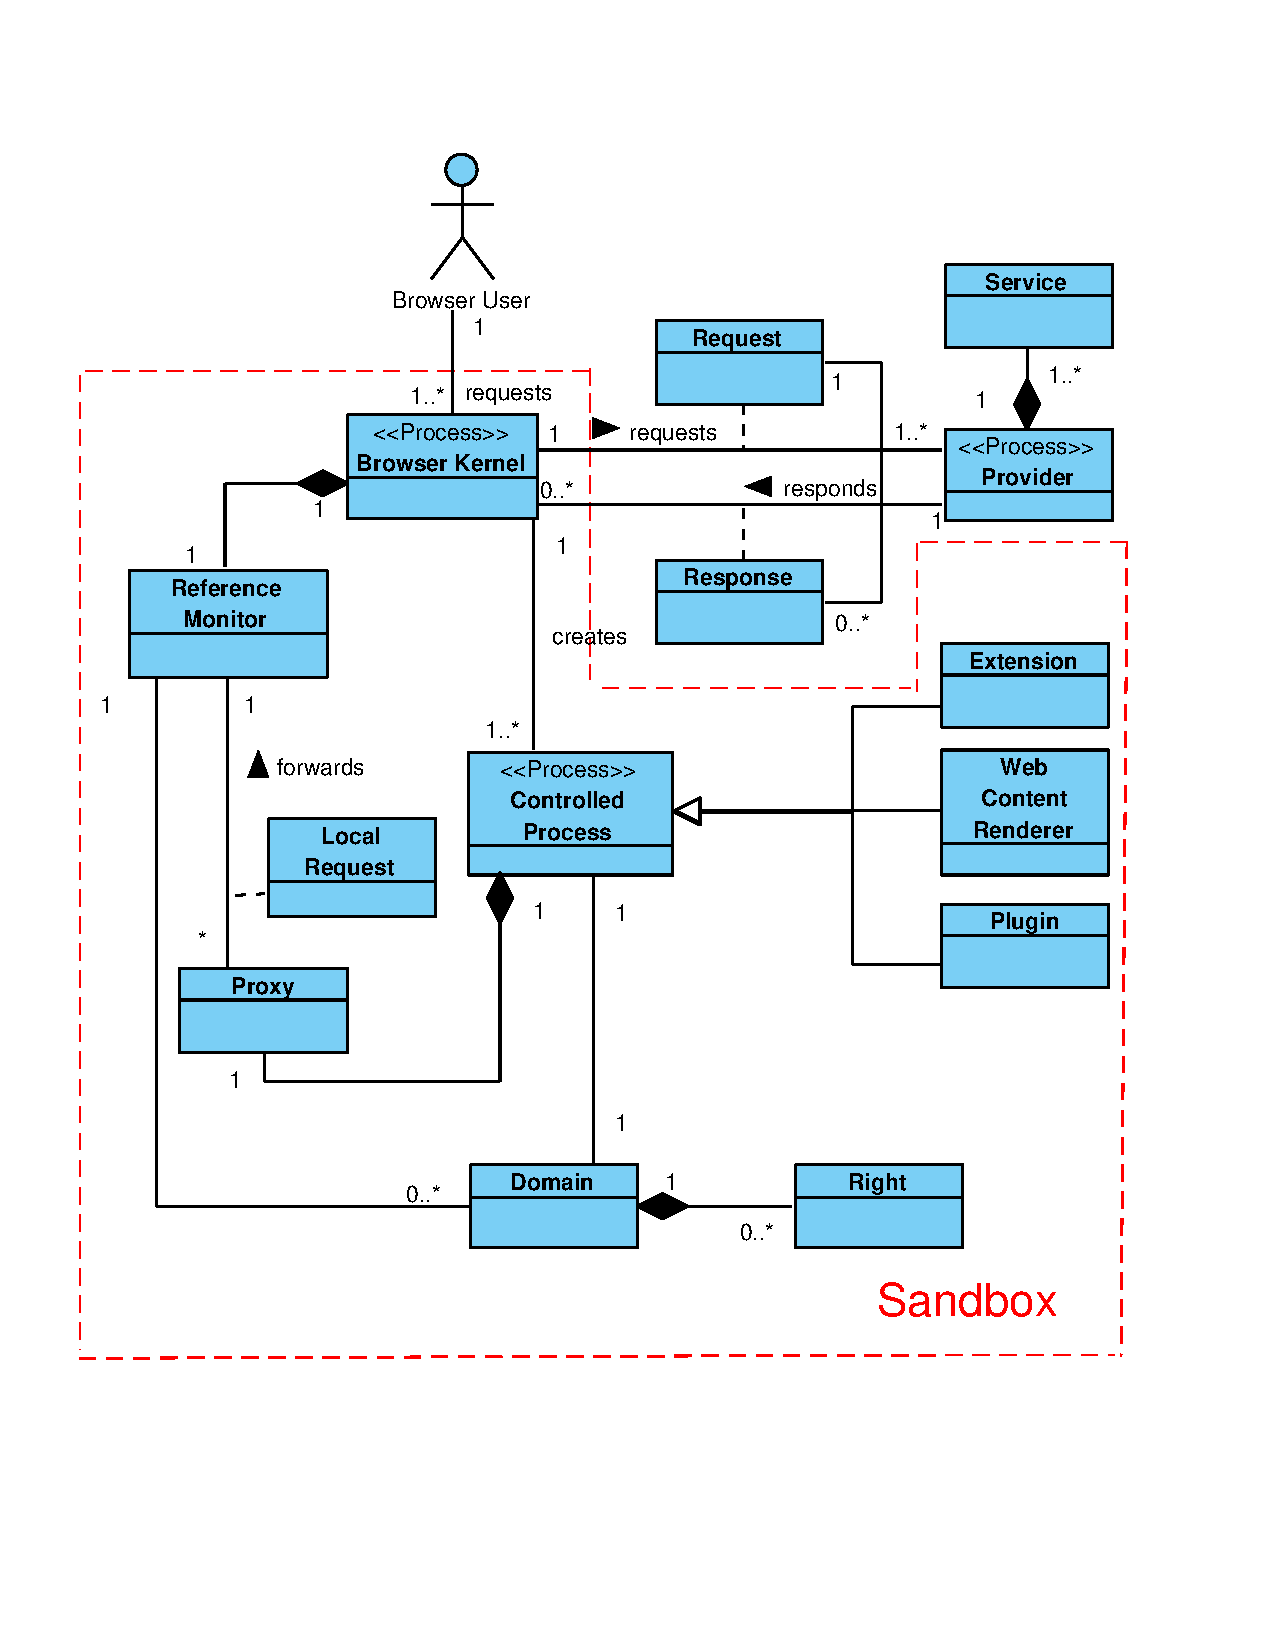
\includegraphics[scale=0.55]{figures/BrowserInfrastructure-v3.pdf}
    %   \vspace*{-2.3cm}
    %   \caption{Web Browser Communication pattern \cite{silva2015}.}
    %   \label{fig:WBCP}
    % \end{figure*}

In this work, a \textbf{Web Browser Content Renderer} pattern is presented (See Figure \ref{fig:relations} to see how it fits with our other patterns). We have already documented a \textbf{Web Browser Communication} pattern \cite{silva2015} as our foundation and in this paper we are extending our RA/SRA with this new pattern. %(Figure \ref{fig:WBCP}). 
The patterns from our RA and SRA were conceived while examining current web browsers like Google Chrome, Internet Explorer and Mozilla Firefox, since these are the most used nowadays. The audience to which our paper is focused are browser developers, web application developers, researchers and teachers, being the first two the most important, since they are the responsible for the implementation and correct use of secure mechanisms. 


\section{Web Browser Content Renderer Pattern}

  \subsection*{Intent}

  The Web Browser Content Renderer describes the architecture for converting the web resources obtained by a browser into a convenient data structure \cite{gpuchrome} or graphical representation, such as a bitmap.%, which will be displayed on the screen to the user.

  \subsection*{Example}
  Once a resource is obtained by the web browser, it is neccesary to interpret it (if the resource is a web page) or save it temporarily or indefinitely in the web browser's host. If it is a web page, the web browser needs to parse it, interpret it and obtain a convenient structure for displaying it on the host's screen.
  
  \subsection*{Context}
  A browser is used to access services or information in the Internet. A browser starts by accepting a URL from a user (explicit request) or an implicit request for interaction with a resource and sending them to the corresponding URL address for that resource or interaction.% and expects an answer. %Web browsers need to parse and interpret the obtained resource to obtain its graphic representation for the user.

  \subsection*{Problem}
  Retrieved resources, such as files, data, images, etc., from providers may be in a specific format; the challenge is to find a way to make them visible on the screen of the user's browser. In this case, if appropriate tools are not available, the resource cannot be helpful because it cannot be seen correctly. How can the host provide these functions? The solution to this problem must resolve the following forces:
  \begin{itemize}\leftskip0.8em
    \item \textit{Transparency}: The user should not be concerned about how a request is manipulated to get its result on the screen.
    \item \textit{Stability}: The browser must be capable of displaying the resource even in the prescence of different formats or syntax errors, like invalid HTML5.
    \item \textit{Isolation}: If a request is completely processed, this is with the browser user permission and should not cause an undesirable behavior with other obtained resources. Also, if an error exists in one resource this should not affect other resources in unexpected ways.
    \item \textit{Heterogeneity}: It does not matter the type of provider with which the browser communicates, it should be possible to interact with any type, and it should be possible to show appropriately the content of the obtained resource.
    \item \textit{Timeliness}: The obtained resource should be displayed within a reasonable time frame; otherwise, a user of the browser would have a bad experience.
  \end{itemize}

  %\begin{shaded}
  \subsection*{Solution}
  Provide the web browser, with the functions needed to understand responses and then obtain a confortable format for the host's Graphics Processor Unit (GPU) to display it to the browser's user. Our solution is directly related to our \textbf{Web Browser Communication} pattern \cite{silva2015} %(Figure \ref{fig:WBCP})
  , where we show the browser's components and the possible interactions between them when a resource is requested. The \textbf{Web Browser Content Renderer} is a specialization of a \textbf{Controlled Process}, and it will communicate with the \textbf{Browser Kernel} of the web browser to do its job, which is rendering a resource.

  %\end{shaded}

  %\begin{shaded}
    \leftskip1em

    \subsubsection*{Structure}
    Figure \ref{fig:WCR} shows a \textbf{Frame Constructor} in charge of building a \textbf{Rendered View} of the requested resource and communicating it to the \textbf{Browser Kernel} %(Figure \ref{fig:WBCP})
    . When a response from a provider needs to be rendered and shown to the user, the \textbf{Frame Constructor} will receive from the \textbf{Browser Kernel} %(Figure \ref{fig:WBCP}) 
    the content of the resource. The \textbf{HTML/XML Parser} is in charge of parsing a web resource and obtain an object representation of it, called a \textbf{DOM Tree} (DOM: Document Object Model). A \textbf{CSS Parser} does the same job as the \textbf{HTML/XML Parser}, but creates \textbf{CSS Style Rules} to change visual aspects of the resource to be displayed. The \textbf{DOM Tree} is a dynamic structure that can change anytime while the resource is needed, by using a scripting language that is interpreted and executed by the \textbf{Javascript Engine \footnote{Since most browsers support Javascript as its scripting language, we have decided using this name}}. \textbf{CSS Style Rules} can also change in the same way, since script languages, like Javascript, can change styles dynamically. A \textbf{Rendered View} is the graphical representation or data structure representing a resource obtained from the \textbf{Browser Kernel} %(Figure \ref{fig:WBCP})
    . A \textbf{Render Tree} is a dynamic structure that links the \textbf{DOM Tree} and \textbf{CSS Style Rules} together, to create a \textbf{Rendered View} or \textbf{bitmap}.

    \subsubsection*{Glossary}
      \begin{itemize}\leftskip0.2em
        \item \textbf{Frame Constructor:} in charge of putting together the results obtained by the parsing process of HTML and CSS files, as well of executing at the right time the Javascript code that will manipulate the DOM Tree and the CSS Styles rules. 
        \item \textbf{Rendered View:} a graphical representation  or data structure of a Render Tree, where this latter was built from the DOM Tree and CSS Style rules obtained from a resource.
        \item \textbf{Bitmap:} a buffer of pixel values in memory (main memory or the GPU’s video RAM) \cite{gpuchrome}.
      \end{itemize}

    \begin{figure*}[h!t]
      %\vspace*{-1.5cm}
      \centering
      %\hspace*{-0.4cm}
      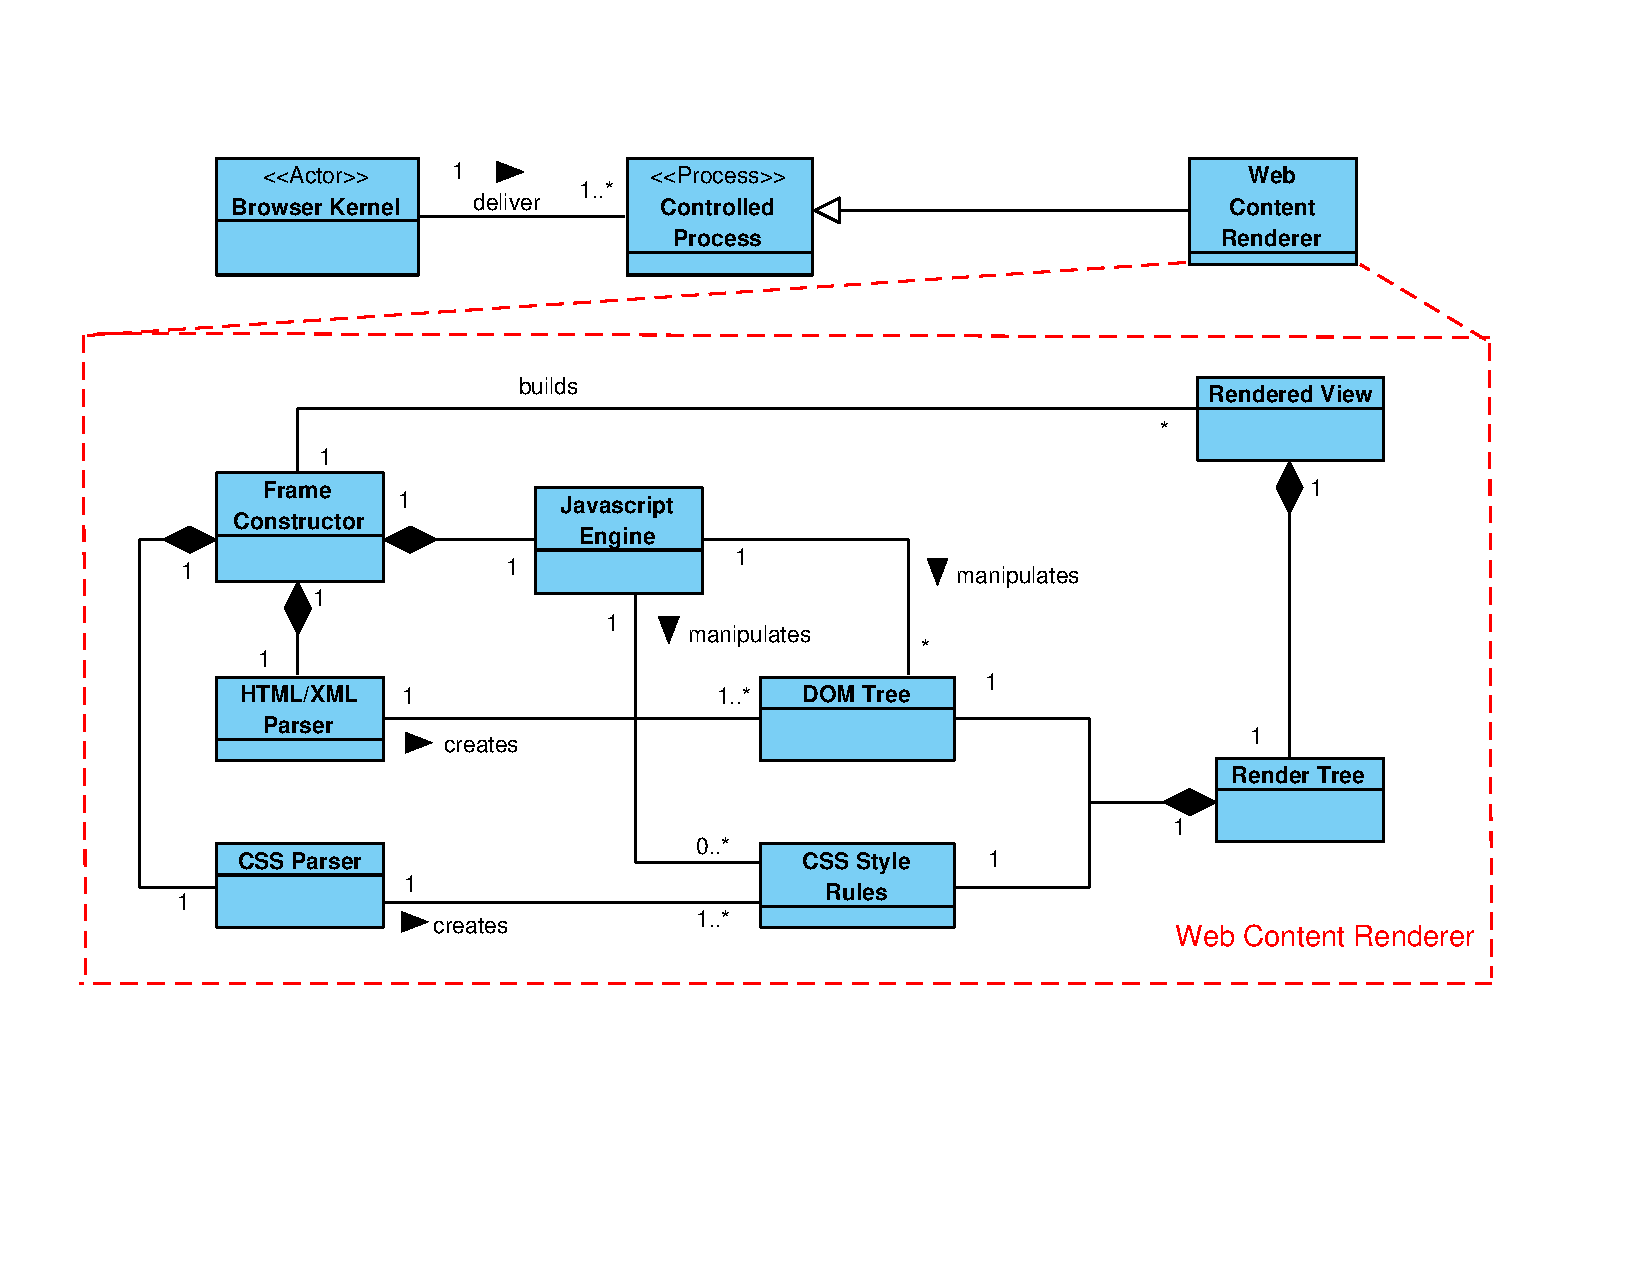
\includegraphics[scale=0.64]{figures/WebContentRenderer-v4.pdf}
      \vspace*{-3cm}
      \caption{High-level Components of the Web Browser Content Renderer.}
      \label{fig:WCR}
    \end{figure*}

    \subsubsection*{Dynamics}
    Some use cases are the following:
    \begin{itemize}\leftskip2.5em
      \item Load Resource (actor: Browser Kernel): which includes the rendering of a resource.

      \item Execute User action (actor: Browser Kernel): changes to the loaded resource done by the user.

    \end{itemize}
    We show below in detail the use case Load Resource. (Figure \ref{fig:LoadResource}):
    \subsubsection*{Summary} The \textbf{Browser Kernel} sends a retrieved resource to the \textbf{Controlled Process} (Figure \ref{fig:WCR})
    , which is instantiated as a \textbf{Web Browser Content Renderer} for displaying the resource appropriately. The resource is obtained by the \textbf{Browser Kernel} from some URL.
    \subsubsection*{Actor} Browser Kernel
    \subsubsection*{Preconditions} In addition to being connected to a network or the Internet, the Host must have one or more \textbf{Browser Kernels}, each one instantiated as a different web browser. Also, the Provider which the browser will contact must be available. 

    \subsubsection*{Description}
      \begin{enumerate}\leftskip2.5em
        \item The \textbf{Browser Kernel} delivers a resource to the \textbf{Controlled Process}, which is instantiated as a \textbf{Web Browser Content Renderer}. The \textbf{Frame Constructor} receives each request for rendering a new resource.
        \item The \textbf{Frame Constructor} uses its \textbf{HTML/XML Parser} to understand the resource. During the parsing process new resources will be needed such as images, plugins, content, etc., where each one of them will perform a Load Resource use case. Step 4 of the sequence diagram in Figure \ref{fig:LoadResource} oversimplifies the request for secondary resources. Where in reality the \textbf{Web Browser Content Renderer} will parallelize loading of secondary resources, or would communicate in a controlled manner (passing through a Reference Monitor) with the \textbf{Browser Kernel} to other \textbf{Controlled Processes} to use plugins or extensions. %(Figure \ref{fig:WBCP})
        \item In parallel the tokenization process creates a dynamic structure called the \textbf{DOM Tree}, which is returned to the Frame Constructor. The same process is done by a \textbf{CSS Parser} to obtain \textbf{CSS Style Rules}.
        \item If scripts are found while parsing the primary resource, the \textbf{Javascript Engine} has the job of parsing, interpreting and executing them. This action can change the \textbf{DOM Tree} and the \textbf{CSS Rules Styles} already built.
        \item Finally, the \textbf{Frame Constructor} is in position for building a convenient data structure or graphical representation of the resource to be rendered. The \textbf{DOM Tree} and \textbf{CSS Styles Rules} are linked together into a \textbf{Render Tree}, and then a process called Layout and Painting is called to get a bitmap \cite{gpuchrome,gecko2} for the \textbf{Browser Kernel}.
      \end{enumerate}

    \subsubsection*{Alternative flows} 
    \begin{itemize}\leftskip2.2em
    \item The HTML/XML Parser fails in getting the \textbf{DOM Tree} from the resource.
    \item The resource does not exist, and an \textbf{Error page} will be created for prompting the user's new action.
    \item The execution of Javascript or the rendering process is cancelled. If the rendering process has not finished, the displaying of the resource will stop.
      \end{itemize}
    \subsubsection*{Postconditions} The \textbf{Browser Kernel} obtains a data structure or graphical representation of the obtained resource.

   % \end{shaded}

    \begin{landscape}
      \begin{figure*}[h!t]
      %\vspace*{-2cm}
          \centering
          \hspace*{-1cm}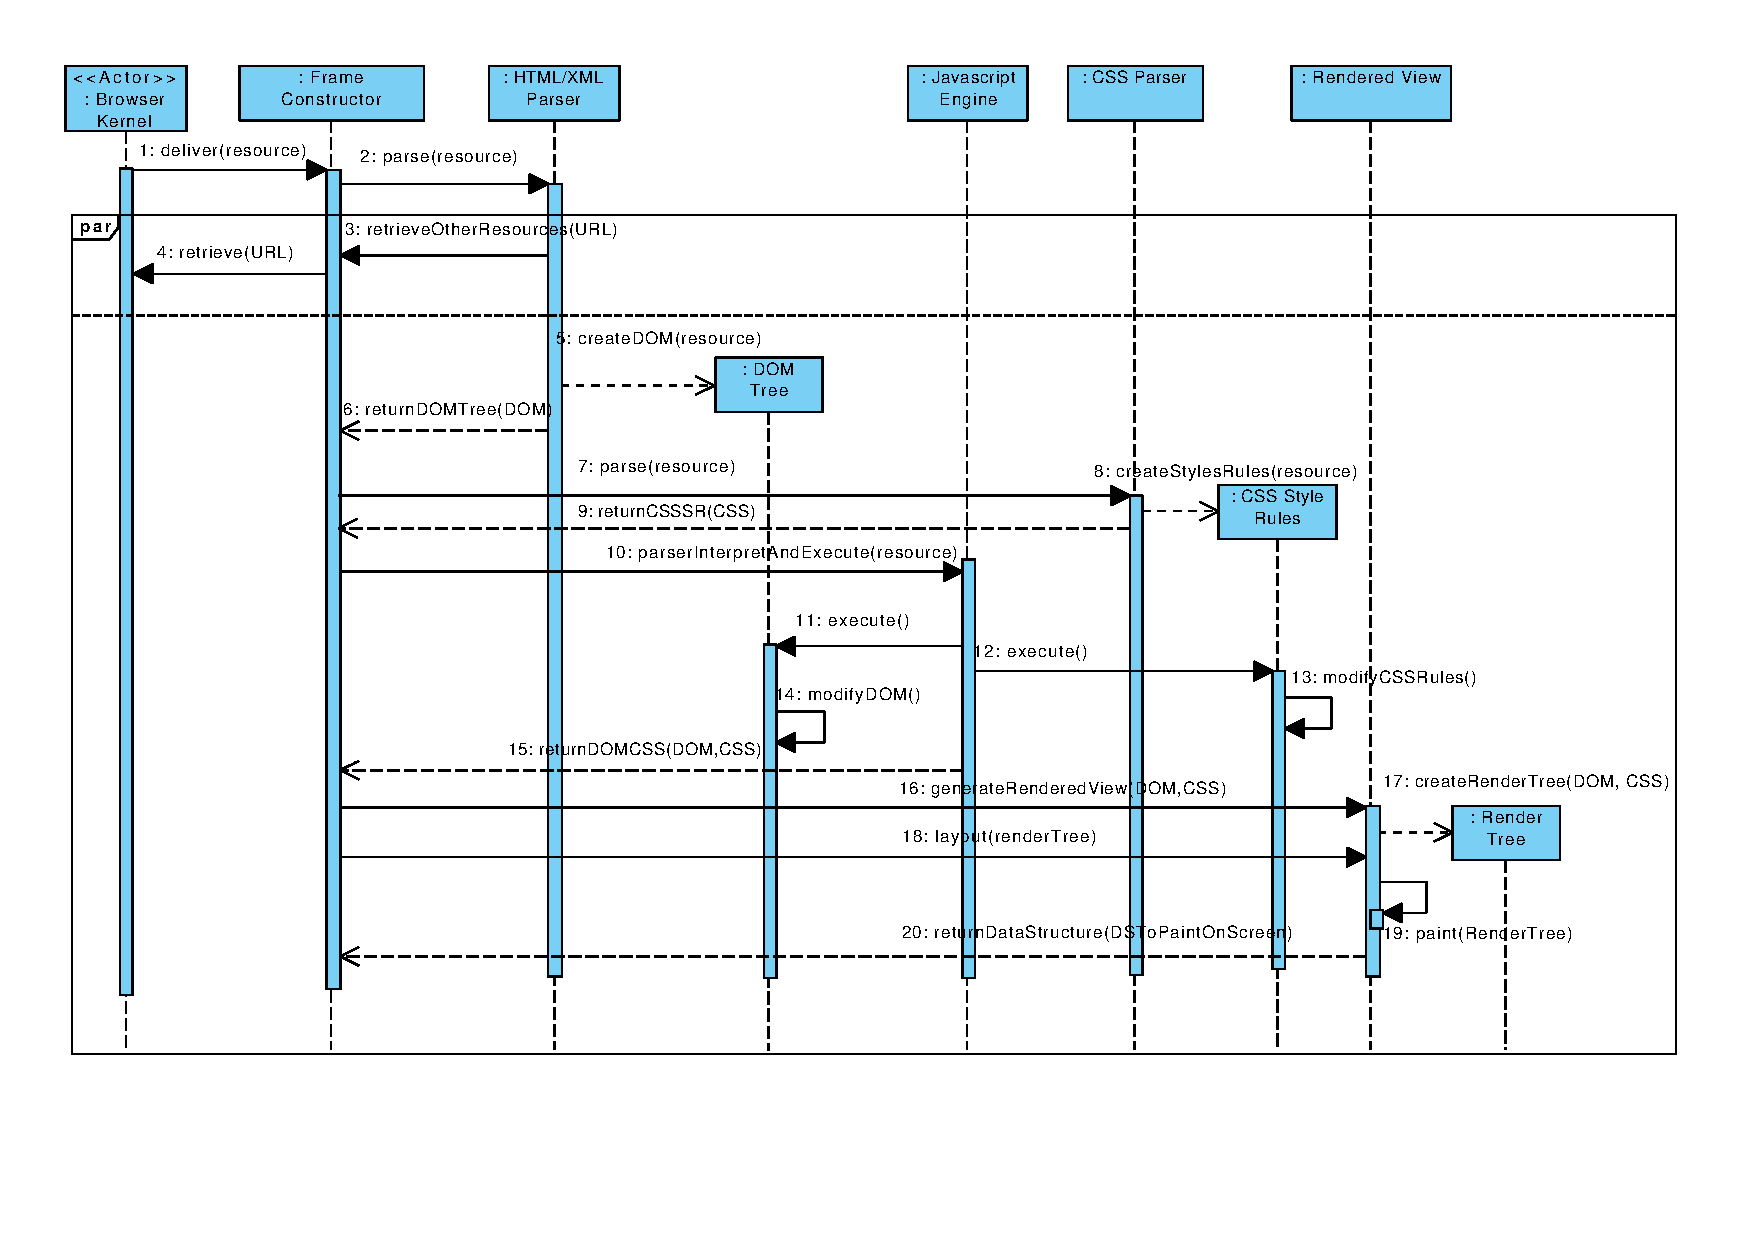
\includegraphics[scale=0.78]{figures/LoadResource-v4.pdf}
          \vspace*{-2.2cm}
          \caption{Sequence Diagram: Load Resource.}
          \label{fig:LoadResource}
      \end{figure*}
    \end{landscape}

    

  \subsection*{Implementation}
    \begin{itemize}\leftskip0.2em
      %\item The Javascript Engine on the Web Browser Content Renderer is normally composed by standard classes, a Javascript Parser that interprets scripting code, a JIT or Just-in-Time Compiler, an Interpreter and a Garbage Collector. Other implementations could have other components, but the must importants are those before \cite{GoogleChromeV8,MicrosoftChakra,MozillaSpidermonkey}.
      \item Most browsers use Javascript for its scripting language. For those who do not use it, it is possible that the rendering engine is only in charge of parsing the resources without building dynamic structures like the DOM, CSS Styles Rules or the Render Tree.
      \item The separation of the components of the \textit{Browser} in various processes, with different levels of access, comes from the more general concept called a Modular Architecture \cite{Vrbanec2013}. This enables the separation of concerns in the browser, which may give greater stability, isolation, security and speed. There are other software architectures used by browsers, but currently the use of a modular architecture is rising.
      \item Each Web Browser Content Renderer instance, is a separate process isolated from others \cite{GoogleChromeIsolation,FirefoxThreatModel}. In this way, the Same Origin Policy (SOP) \cite{W3C-SOP} is enforced in each instance defined by the origin of the resources: by their domain, scheme and port. The mentioned policy is the minimum security mechanism a browser has while requesting cross-origin resources, and divides the different kind of contents, avoiding mutual interference. To enforce the SOP, Google Chrome, Firefox and Internet Explorer use different schemes \cite{Crowley2010,Reis2009,Jackson2008}.
      \item Google Chrome and Internet Explorer have their rendering engine implemented with a sandbox mechanism. This security feature makes every renderer instance to have restricted privileges on the system, so they cannot interact in a dangerous way with the system. This defense mechanism enforces a least privilege policy, so the file system can be safe against threats that try to exploit web page vulnerabilities.
    \end{itemize}



  \subsection*{Consequences}
  \leftskip-0.1em The Web Browser Content Renderer pattern provides the following benefits:
  \begin{itemize}\leftskip0.2em
    \item \textit{Transparency}: The process for rendering a resource is done without user interaction.
    \item \textit{Stability}: Even if a resource (HTML for example) is invalid, the rendering process will try to get a visual representation. Another type of resource could be handled the same way or by requesting again the resource. Since a Web Browser Content Renderer instance is separate process, each has its own memory space, even if an error is found while loading a resource it will not affect the whole browser and will be able to continue working.
    \item \textit{Isolation}: Resources are placed in different processes (different memory spaces) and can only interact if the Same Origin Policy allows it. A Reference Monitor for the DOM Tree and Capabilities for the Javascript Engine are used to enforce this policy (Same Origin Policy - SOP). If a Web Browser Content Renderer makes an error while loading or processing a resource, it will not affect other processes that have instantiated the Web Browser Content Renderer pattern that are part of the same browser.
    \item \textit{Heterogeneity}: Because each web browser tries to follow the standards of the W3C \cite{w3c}, every page that follows these guidelines can be viewed, independent of the type of browser.
    \item \textit{Timeliness}: Since a renderer engine will be in charge of rendering a particular page or pages (if bound by the SOP as in Google Chrome), the time it will take to load several resources in differents renderer engines will be less compared to the worst case when only one renderer is used for the same task.
  \end{itemize}
  This pattern has the following liabilities:
  \begin{itemize}\leftskip0.2em
    \item Since many independent processes are used to create a Web Browser Content Renderer for rendering a resource (depending on the scheme using the browser), it is possible that a lot of the host's resources are used to keep everything active. A modular architecture requires heavier data structures for multiprocessing and keeping all processes working, compared with a monoprocess architecture with multithreading.
    \item Resources from providers which do not comply with the specifications of the W3C, will be displayed incorrectly by the web browser.
  \end{itemize}

  \subsection*{Example Resolved}
With the given pattern it is now possible to display content to the user and/or navigate smoothly through the obtained resources. Independent of the type of web resource, it will be possible to obtain an abstraction of it and display it appropriately in the browser. 
  \subsection*{Known Uses}
  \begin{itemize}\leftskip0.2em
    \item Google Chrome is based on a modular architecture, where each Renderer Process communicates with the Browser Kernel \cite{multiProcGC}. Blink is the implementation of its renderer engine and is based on WebKit.
    \item Gecko \cite{gecko2} is the name for the Renderer in the monoprocess architecture of Firefox, it is written in C++ and can be used to render the user interface of other applications such as Thunderbird.
    \item Internet Explorer, a proprietary browser, does not give much information about its structure or details of its implementation; \cite{Crowley2010} addresses Loosely-Coupled architecture \cite{IE8-LCIE} and its components, like Trident its Rendering Engine, but without giving further details. Microsoft's new web browser, Microsoft Edge, integrates a new renderer, called EdgeHTML \cite{edgehtml}.
  \end{itemize}

  \subsection*{Related Patterns}
  \begin{itemize}\leftskip0.2em
    \item The Web Browser Communication pattern presents the components of the web browser and how they communicate with each other when a resource is requested \cite{silva2015}. 
    \item The Reified Reference Monitor \cite{fernandez2013security}, describes how to enforce authorization rights when a subject requests access to a protected object or service and returns a decision (response). 
    \item The Client Rendering Pattern by Vilar et. al \cite{Vilar2015} (which proposed five patterns to organize GUI widgets based on domain model meta data), resolves the problem of developers to compose widgets indirectly in the client layer of web Enterprise applications. The Rendering Engine, which is represented here as the Web Browser Content Renderer, is part of the architecture diagram for the Client Rendering Pattern.
  \end{itemize}

\section{Conclusions and Future Work}
A web browser appears to be a medium complexity software for users and developers without security experience. Unfortunately, this software allows a variety of attack vectors, to the user as well as to the system with which interacts. Therefore, it is important to understand its structure and how it interacts with internal and external stakeholders.

A first part of our RA has been formulated with the \textbf{Web Browser Communication} pattern, and now we have presented our second architectural pattern: the \textbf{Web Browser Content Renderer}. These two patterns abstract the infrastructure of a web browser to help others understand holistically the components, interactions and relationships of this system. 
%Furthermore, it has been possible to characterize the stakeholders and one of the most important use cases, the \textbf{Load Resource} use case. From what we know, our current proposal is the second Reference Architecture for the web browsers. The reference model obtained in \cite{2005-grosskurth-browser-refarch} describes the type of architecture used in the nineties until 2009 (approximately). However, our proposal represents the current implementation used in browsers, a \textit{Modular Architecture}. 
The proposed work allows a better understanding of browser's structure and behavior within our partial Reference Architecture, which is also helpful to understand existing threats in the browser. Furthermore, since a pattern is generic by definition, our solution is not tied to specific implementations and is possible to generalize some results to other browsers. 

As a we are finishing a complete Reference Architecture for web browsers, another pattern related to the Web Browser Communication pattern will be obtained in order to complete the Reference Architecture, called the Browser Kernel pattern. 

We plan to build more \cite{silva2015b} misuse patterns for the Web Browser Communication pattern, to continue the study of the possible threats in the \textit{Browser}, as a way to educate developers and stakeholders. At the same time, these patterns will allow the construction of a Security Reference Architecture for the browser. In the same line, in addition to finding potential threats in the system, we need to find countermeasures to prevent or foresee such threats through security patterns on the reference architecture. An example of the type of work to be carried out can be seen in \cite{Fernandez2016}.

\section{Acknowledgements}
We thank our shepherd, Christopher Preschern, for his useful comments that significantly improved the quality of the paper. We also thank Elissaveta Gourova for supervising our paper shepherding. We
would also like to gratefully thank to the participants of the EuroPLoP Writers Workshop: Tobias Rauter, Veli-Pekka Eloranta, Poonam Ponde, Shailaja Shirwaikar, Bogdana Botez, Andreas Sinnhofer, Roland H. Steinegger, Lukas Reinfurt. This work was partially supported by CONICYT (grant Fondecyt 1140408).





\bibliographystyle{ACM-Reference-Format-Journals}
\bibliography{refTodas}  
\end{document}
